\chapter{Quantifying Uncertainty : Measurement of Gravitational Acceleration}

Date: 5/9/2020

\section{Aim}

In this experiment, our aim is to measure the gravitational acceleration of Earth using a pendulum and quantify various Type A and Type B uncertainties to produce a concrete uncertainty of our measurement. We observe the relationship between the Length of a pendulum and its Time Period. We use a metallic bob with a hook as our pendulum.

\section{Background Theory}

Newton's Law of Gravitation states that `' Any particle of matter in the universe attracts any other with a force varying directly as the product of the masses and inversely as the square of the distance between them. '' Mathematically, it can be expressed as 
$$\vec{F} = -G \frac{m_1 \times m_2}{r^2} \hat{r}$$
where G is the gravitational constant, $m_1$ is the mass of body 1, $m_2$ is the mass of body 2 and $r$ is the separation between the center of masses of both bodies. Newton's second of motion states ``that rate of change of momentum of a body is directly proportional to the force applied'' which can be expressed in the form 
$$ \vec{F} = m \times \vec{a}$$
where m is the mass of the body and a is the acceleration. Combining these both Laws, gives us the following equation
$$ g = -G \frac{M_E}{{R_E}^2} $$
where the $M_E$ is the mass of the Earth and $R_E$ is the radius of the Earth.\\
The length (L) of the pendulum is related to its time period (T) by the following equation:
$$ T = 2\pi\sqrt{\frac{L}{g}} $$
This equation can be re-written by making g the subject :
$$ g = 4\pi^2\frac{L}{T^2} $$

\section{Description of Setup}
% \begin{figure}[h!]
%     \centering
%     \includegraphics[width=\textwidth]{figures/A1.png}
%     \caption{Apparatus}
%     \label{fig:yx}
% \end{figure}
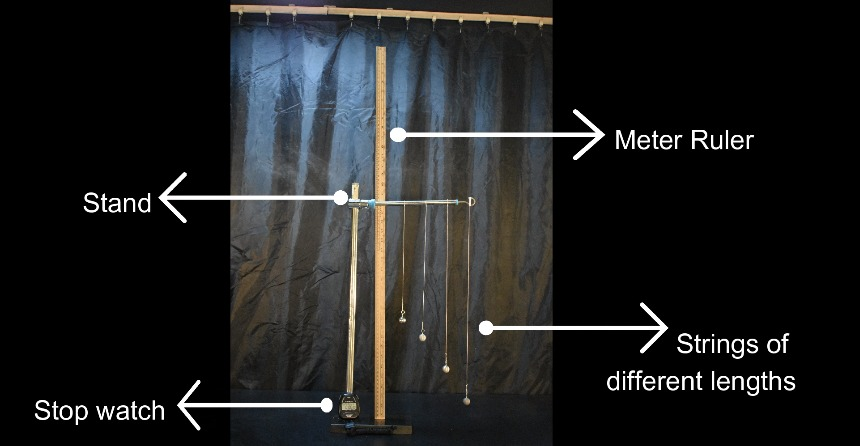
\includegraphics[width=10cm, height=8cm]{figures/fig1g.jpeg} \\
Here the stand with clamp is used to provide a rigid support, metre rule is used to measure the length L of the pendulum , digital stopwatch is used to record the time period of the pendulum and the metallic bob with a hook is used as a pendulum. In this experiment, we use four different length of threads


\section{Method / Procedure}

The length of the thread is measured from the clamp to the center of the metallic bob using the metre Ruler. Digital stopwatch is used to record the time-period for ten oscillations. The same process is repeated 5 times for each  thread. Length of the Pendulum is adjusted by attaching the metallic bob to a thread of different length.Threads of four different lengths are used in this Experiment. \\
The gravitational acceleration $g_i$ is calculated for each different length of pendulum by using the average time period of one oscillation and theory described above. These $g_i$'s are then combined together to calculate the final value of the gravitational acceleration $g$.

\section{Data}

Since the length of the pendulum was only measured it has no type A uncertainty. The type B uncertainty associated with the metre ruler and digital stopwatch are $0.0002m$ and $0.003s$ \\
The lengths of the Pendulum measured using the metre ruler.
\begin{center}
\begin{tabular}{|c|c|c|c|c|c|}
\hline
\textbf{s.No} & \textbf{Height} & \textbf{Upper (cm)} & \textbf{Lower (cm)} & \textbf{Length (cm)} & \textbf{Length (m)} \\ \hline
1             & H1              & 80.7                & 43.0                & 37.7                 & $0.377 \pm 0.0002 $ \\ \hline
2             & H2              & 73.5                & 42.3                & 31.2                 & $0.312 \pm 0.0002 $ \\ \hline
3             & H3              & 68.0                & 42.7                & 25.3                 & $0.253 \pm 0.0002 $ \\ \hline
4             & H4              & 92.7                & 42.0                & 50.7                 & $0.507 \pm 0.0002$ \\ \hline
\end{tabular}
\end{center} 
The time period for ten-oscillations recorded using digital stopwatch.
\begin{center}
\begin{tabular}{|c|c|c|c|c|}
\hline
\textbf{s.No} & \textbf{T\_H1 (s)} & \textbf{T\_H2 (s)} & \textbf{T\_H3 (s)} & \textbf{T\_H4 (s)} \\ \hline
1             & 11.60              & 11.53              & 10.22              & 14.62              \\ \hline
2             & 11.40              & 11.18              & 10.19              & 14.50              \\ \hline
3             & 11.10              & 11.21              & 10.22              & 14.41              \\ \hline
4             & 11.30              & 11.25              & 10.28              & 14.47              \\ \hline
5             & 11.30              & 11.31              & 10.44              & 14.60              \\ \hline
\end{tabular}
\end{center}
Type A uncertainty in the Time Period for each length was calculated using the method mentioned in the MATLAB script . \\
Type A uncertainty in Time Period for H1
\begin{center}
$\sigma_T = 0.0162 s$ \\
$ U_T^A =  0.0081s$ \\
\end{center}
$ U_T = \sqrt{{U_T^A}^2 +{U_T^B}^2}$ \\
$ U_T = \sqrt{0.0081^2+0.003^2}$ \\
$ U_T = 0.0086s $ \\
Total uncertainty in Time Period (T1)  for $H_1$ is $ T = 1.134 \pm 0.009 s$\\
Type A uncertainty in Time Period for H2
\begin{center}
$\sigma_T = 0.0125 s$ \\
$ U_T^A =  0.0062s$ \\
\end{center}
$ U_T = \sqrt{{U_T^A}^2 +{U_T^B}^2}$ \\
$ U_T = \sqrt{0.0062^2+0.003^2}$ \\
$ U_T = 0.0069s $ \\
Total uncertainty in Time Period (T2)  for $H_2$ is $ T = 1.130 \pm 0.007 s$\\
Type A uncertainty in Time Period for H3
\begin{center}
$\sigma_T = 0.090 s$ \\
$ U_T^A =  0.0045s$ \\
\end{center}
$ U_T = \sqrt{{U_T^A}^2 +{U_T^B}^2}$ \\
$ U_T = \sqrt{0.0045^2+0.003^2}$ \\
$ U_T = 0.0053s $ \\
Total uncertainty in Time Period (T3) for $H_3$ is $ T = 1.027 \pm 0.005 s$\\
Type A uncertainty in Time Period for H4
\begin{center}
$\sigma_T = 0.079 s$ \\
$ U_T^A =  0.0040s$ \\
\end{center}
$ U_T = \sqrt{{U_T^A}^2 +{U_T^B}^2}$ \\
$ U_T = \sqrt{0.0040^2+0.003^2}$ \\
$ U_T = 0.0049s $ \\
Total uncertainty in Time Period (T4)  for $H_4$ is $ T = 1.452 \pm 0.005 s$
    
\section{Data Analysis}
The formula for calculating g is as follows :
$$ g = 4\pi^2\frac{L}{T^2} $$
Transferring the uncertainty in Time and Length to gravitational acceleration
$$ U_g = \sqrt{\Bigg({4\pi^2 \frac{(-2)L}{T^3} \Delta T}\Bigg)^2+\Bigg({4\pi^2 \frac{1}{T^2} \Delta L}\Bigg)^2}$$
$$ U_g = \frac{4\pi^2}{T^2} L \sqrt{ {\bigg( \frac{-2 \Delta T}{T}  \bigg)}^2    +  {\bigg( \frac{\Delta L}{L} \bigg)}^2} $$

$$ U_g = g\sqrt{ {\bigg( \frac{-2 \Delta T}{T}  \bigg)}^2    +  {\bigg( \frac{\Delta L}{L} \bigg)}^2} $$
Calculating g1 
$$ g_1 = 4\pi^2 \frac{L_1}{{T1}^2} = 4\pi^2 \frac{0.377}{{1.134}^2}  = 11.5738  m/s^2 $$ 
$$ \sigma_1 = 11.5738 \sqrt{{\bigg(\frac{-2 \times 0.009}{1.134}\bigg)}^2+{\bigg(\frac{0.0002}{0.377}\bigg)}^2} = 0.1761  m/s^2 $$
$$ g = 11.5738 \pm 0.1761 m/s^2 $$
Calculating g2
$$ g_2 = 4\pi^2\frac{L_2}{{T2}^2} = 4\pi^2 \frac{0.312}{1.130^2}  = 9.6531  m/s^2  $$ 
$$ \sigma_2 = 9.6531 \sqrt{{\bigg(\frac{-2 \times 0.007}{1.130}  \bigg)}^2+{\bigg( \frac{0.0002}{0.312} \bigg)}^2} = 0.1155 m/s^2 $$
$$ g = 9.6531 \pm 0.1155 m/s^2$$
Calculating g3
$$ g_3 = 4\pi^2\frac{L_1}{{T1}^2} = 4\pi^2 \frac{0.253}{{1.027}^2}  = 9.4698 m/s^2$$ 
$$ \sigma_3 = 9.4698 \sqrt{{\bigg( \frac{-2 \times 0.005}{1.027} \bigg)}^2+{\bigg( \frac{0.0002}{0.253} \bigg)}^2} = 0.0988  m/s^2 $$
$$ g = 9.4698 \pm 0.0988 m/s^2 $$
Calculating g4
$$ g_4 = 4\pi^2\frac{L_1}{{T1}^2} = 4\pi^2 \frac{0.5070}{1.452^2}  = 9.4937  m/s^2 $$ 
$$ \sigma_4 = 9.4937 \sqrt{ {\bigg( \frac{-2 \times 0.005}{1.452}  \bigg)}^2    +  {\bigg( \frac{0.0002}{0.5070} \bigg)}^2} = 0.0642 m/s^2$$
$$ g = 9.4937 \pm 0.0642 m/s^2$$
Now we can combine the $g1,g2,g3$ and $g4$ and their uncertainties to obtain the final value for gravitational acceleration and its uncertainty.

$$ g = \frac{ (\frac{g_1}{{\sigma_1}^2}+\frac{g_2}{{\sigma_2}^2}+\cdots)} {(\frac{1}{{\sigma_1}^2}+\frac{1}{{\sigma_2}^2}+\cdots)} = \frac{\sum_{i} \frac{g_i}{{\sigma_i}^2} }{\sum_{i} \frac{1}{{\sigma_i}^2} }$$
Combining the uncertainties in $g1,g2,g3$ and $g4$
$$ \sigma^2 =  \frac{1}{\sum_{i} \frac{1}{{\sigma_i}^2} }$$

$$ g = 9.6631  \pm 0.0472 m/s^2$$





\section{Discussion \& Conclusion}

The percentage uncertainty is 0.98 \%, and standard value of gravitational acceleration is not in the range $ g = 9.6631  \pm 0.0472 m/s^2$. Possible factors of uncertainty and errors are external factors such as wind and human errors in recording final time. Therefore there is a chance that hypothesis is not valid since standard value is not in the range. Perhaps a more accurate set up could have given results that would agree with hypothesis. Improvement can be a more accurate mechanism for recording time such as light gate, we can also ensure that external factors such as wind are minimized by using wind blockers and we can also use a fiducial marker to mark the mean of an oscillation. 

% Summarize and discuss the experimental results, what do the results say about your hypothesis, if such a hypothesis was made for the experiment. Mention the uncertainty in the calculated quantity Be precise and only include scientific discussion.


\section{MATLAB Script}
\lstinputlisting{matlabCodes/Experiment1.m}



